\chapter{Công trình nghiên cứu liên quan}
\label{chap:chap2}
\section{Graph neural networks}

\begin{figure}
    \centering
    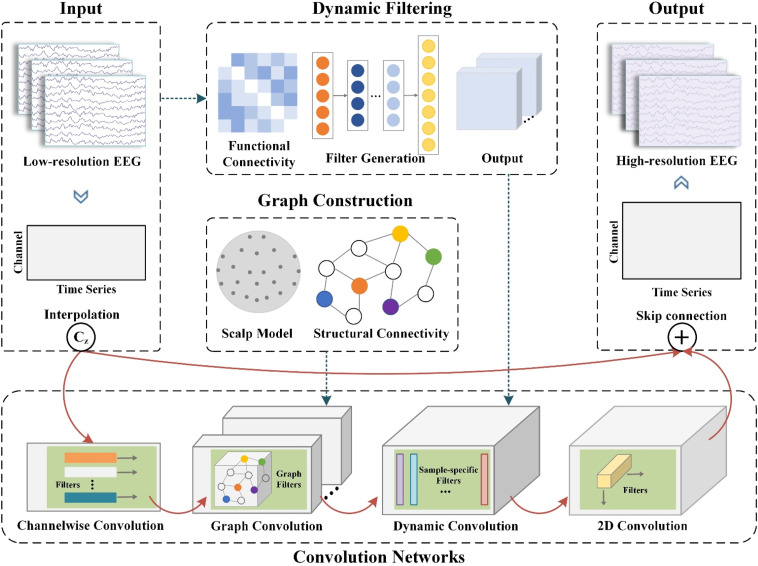
\includegraphics[width = 0.8\textwidth]{imgs/graph-convolutional-networks.jpg}
    \caption{Minh hoạ cấu trúc graph convolutional networks}
    \label{fig:CF_CBF}
\end{figure}
Mạng đồ thị (Graph Networks) là một khái niệm trong lĩnh vực trí tuệ nhân tạo và học máy. Các thực thể riêng lẻ trong mạng đồ thị không chỉ được xem xét độc lập, mà mối quan hệ giữa chúng còn được coi trọng không kém bản thân các thực thể đó. Theo Battaglia và cộng sự (2018) \cite{battaglia2018relational}, các thực thể chính là các nút (nodes), và những mối liên kết tương tác giữa chúng là các cạnh (edges). Cấu trúc này cho phép chúng ta nắm bắt được sự phụ thuộc lẫn nhau và các tương tác phức tạp, điều mà các mô hình truyền thống thường bỏ qua.

Một hiện thực tiêu biểu và đang phát triển mạnh mẽ của cách tiếp cận này là Mạng Nơ-ron Đồ thị (Graph Neural Networks - GNNs). GNNs thực chất được sử dụng chủ yếu cho dữ liệu có cấu trúc dạng đồ thị. Sức mạnh cốt lõi của GNNs nằm ở khả năng truyền tải và kết hợp thông tin giữa các nút nhờ vào các mối liên kết trên đồ thị. Quá trình này giúp GNNs học được những biểu diễn dữ liệu vô cùng phong phú và có ý nghĩa cấu trúc tổng thể của toàn bộ đồ thị. Nhờ vậy, GNNs được sử dụng để phân tích các mối quan hệ trong mạng xã hội, dự đoán hành vi người dùng hoặc xây dựng các hệ thống khuyến nghị cá nhân hóa \cite{wu2022graph, gao2022hetinf, min2021stgsn}.

Bên cạnh các ứng dụng đã được khẳng định trong phân tích mạng xã hội và hệ thống khuyến nghị, một hướng ứng dụng khác của GNNs, đặc biệt là trong bối cảnh dữ liệu thực tế, là bù đắp (imputation) các giá trị khuyết trong dữ liệu đồ thị. GNNs có thể khai thác toàn bộ cấu trúc đồ thị, đây là một điểm nổi bật và vượt trội. Thay vì chỉ xử lý từng điểm dữ liệu một cách độc lập hoặc cục bộ, GNNs tích hợp thông tin từ cấu trúc tổng thể của đồ thị. Điều này cho phép GNNs suy diễn và điền các giá trị thiếu với độ chính xác cao hơn hẳn, bởi vì chúng không chỉ dựa vào dữ liệu có sẵn mà còn tính đến các mối quan hệ giữa các thực thể. Nhờ vậy, GNNs có khả năng tích hợp thông tin, đồng thời học được các biểu diễn tiềm ẩn phản ánh sâu sắc cấu trúc nội tại của dữ liệu.

Tiềm năng của các phương pháp dựa trên GNNs đã được chứng thực qua nhiều nghiên cứu thực tiễn. Một minh chứng tiêu biểu là công trình của Spinelli và cộng sự (2020) \cite{spinelli2020missing}, trong đó các tác giả đã cho thấy hiệu quả của việc áp dụng GCNs – một biến thể phổ biến của GNNs – để xử lý dữ liệu thiếu trong các lĩnh vực phức tạp như ô nhiễm môi trường, y tế và khoa học vật lý. Những kết quả tích cực này tạo ra một cơ sở khoa học vững chắc, gợi mở tiềm năng ứng dụng GCNs vào lĩnh vực giáo dục, đặc biệt là để cải thiện chất lượng dữ liệu cho các khóa học trực tuyến mở (MOOCs).

Tóm lại, năng lực vượt trội của GNNs trong phân tích mạng xã hội và các lĩnh vực khác đã được làm rõ. Năng lực này càng trở nên nổi bật khi GNNs thể hiện lợi thế vượt trội, đặc biệt đối với bộ dữ liệu thưa thớt. Khả năng đặc biệt này đã giúp cho GNNs trở nên phù hợp với bài toán của các khóa học trực tuyến mở (MOOCs). Trong môi trường MOOC, việc thu thập dữ liệu hành vi người học thường gặp phải nhiều gián đoạn, dẫn đến dữ liệu không đầy đủ. GNNs mang đến một giải pháp tiềm năng để biến những bộ dữ liệu tưởng chừng "khuyết tật" này thành nguồn tài nguyên giá trị, từ đó giúp các mô hình học sâu đưa ra những phân tích và dự đoán chính xác hơn.


% % Trong nghiên cứu này, các mô hình khuyến nghị được đề cập đều được xây dựng dựa trên kiến trúc Transformer, một mạng nơ-ron sâu đã tạo nên bước đột phá trong lĩnh vực xử lý ngôn ngữ tự nhiên (NLP) \cite{transformer}. Kể từ ngày được công bố, Transformer đã dần trở thành một chuẩn mực trong nhiều lĩnh vực khác nhau, trong đó có các hệ thống khuyến nghị. Nhờ vào khả năng vượt trội trong việc nắm bắt các mối quan hệ phức tạp trong dữ liệu với cốt lõi là cơ chế attention, đặc biệt là self-attention, cho phép Transformer xử lý thông tin một cách song song và hiệu quả, không bị giới hạn bởi các ràng buộc tuần tự như trong các mô hình \gls{RNNs} truyền thống. Điều này giúp Transformer có thể hiểu rõ hơn về ngữ cảnh và ý nghĩa của dữ liệu, từ đó đưa ra các dự đoán và gợi ý chính xác hơn. 
% % % \begin{figure}[t]
% % %     \centering
% % %     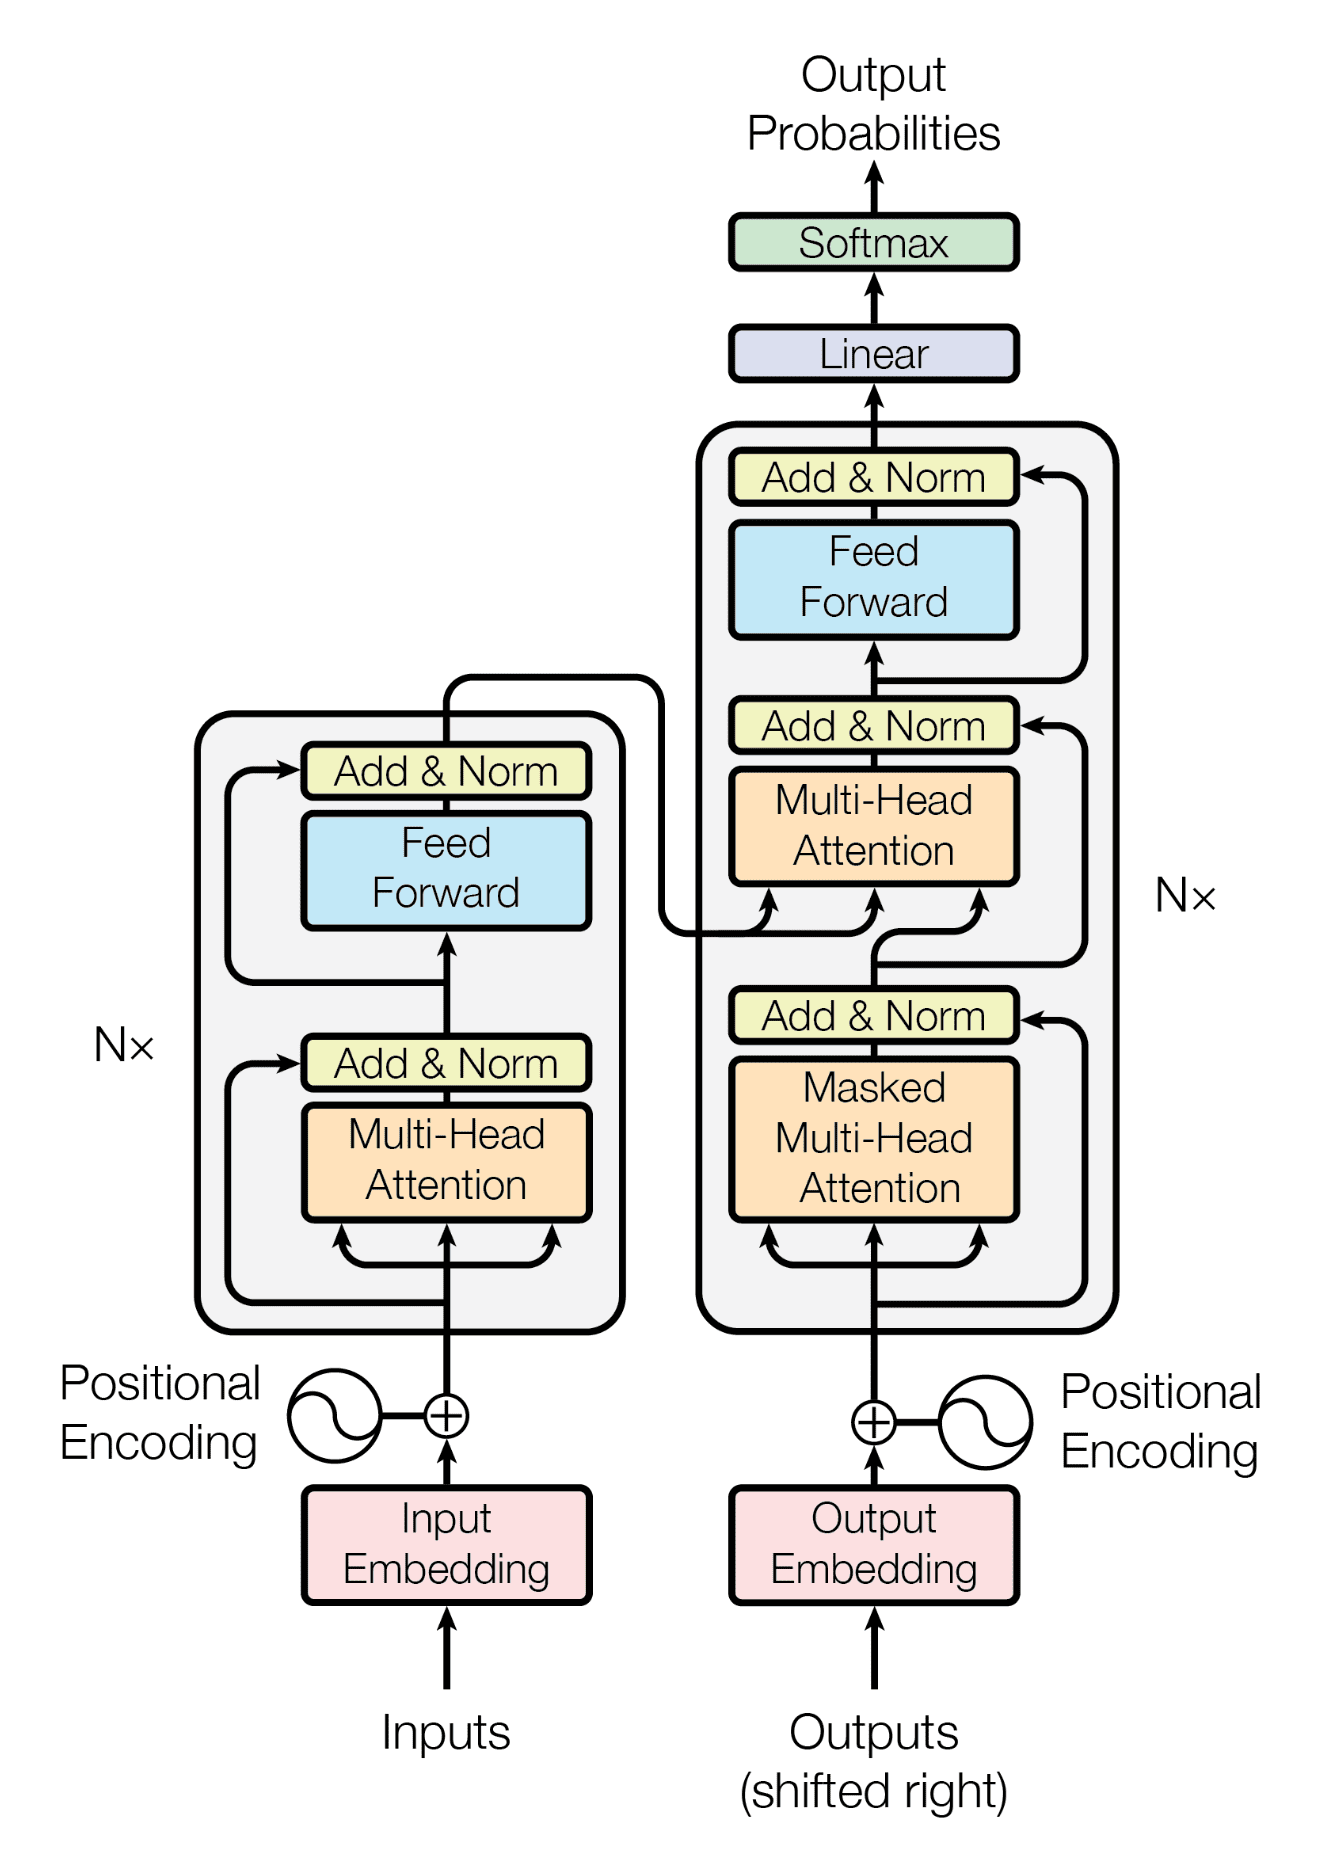
\includegraphics[width = 0.5\textwidth]{imgs/attention_research_1.png}
% % %     \caption{Kiến trúc Transformer}
% % %     \label{fig:transformer}
% % % \end{figure}
% % Như hình \ref{fig:transformer}, Transformer gồm hai thành phần chính: Encoder và Decoder. Tuy nhiên, trong nhiều ứng dụng như hệ thống khuyến nghị, chỉ thành phần Encoder được sử dụng.
% % \subsubsection{Encoder}
% % Encoder của Transformer bao gồm một số lớp lặp lại, mỗi lớp bao gồm hai thành phần chính:
% % \begin{itemize}
% %     \item \textbf{Cơ chế Multi-Head và Self-Attention:} Là cốt lõi của Transformer. Cơ chế này cho phép mỗi phần tử trong chuỗi đầu vào tự đánh giá mức độ quan trọng của mình so với các phần tử khác, từ đó xác định mối liên hệ và ảnh hưởng lẫn nhau. Nhờ vậy, Transformer có khả năng nắm bắt đồng thời nhiều loại quan hệ khác nhau, từ gần đến xa, giúp mô hình hiểu rõ hơn về cấu trúc và ngữ nghĩa của dữ liệu.
% %     \item \textbf{Feed-Forward Neural Network:} Sau khi áp dụng self-attention, kết quả đầu ra được đưa đến một mạng nơ-ron chuyển tiếp. Mạng này gồm hai lớp nơ-ron với hàm kích hoạt phi tuyến, đóng vai trò như một bộ lọc giúp học được các đặc trưng phức tạp và trừu tượng từ dữ liệu.
% % \end{itemize}
% % Mỗi lớp trong Encoder cũng có các cơ chế chuẩn hóa và cơ chế dropout để cải thiện tính ổn định và giảm thiểu hiện tượng overfitting.

% % \subsubsection{Decoder}
% % Mặc dù không thường xuyên suất hiện trong các hệ thống khuyến nghị, nhưng thành phần Decoder của Transformer cũng bao gồm các lớp multi-head attention và feed-forward tương tự như trong Encoder. Điểm khác biệt chính nằm ở cơ chế attention đặc biệt của Decoder, cho phép nó tương tác với đầu ra của Encoder. Nhờ đó, Decoder có thể tổng hợp thông tin từ cả dữ liệu đầu vào và ngữ cảnh hiện tại, từ đó đưa ra những dự đoán chính xác và phù hợp hơn.

% % \subsubsection{Self-Attention và Multi-Head Attention}
% % Cơ chế self-attention là một trong những yếu tố cốt lõi làm nên sức mạnh của Transformer. Nó cho phép mô hình tự động tập trung vào những phần quan trọng của dữ liệu đầu vào bằng cách tính toán một bộ trọng số thể hiện mức độ liên quan giữa các phần tử trong chuỗi. Công thức cho self-attention bao gồm ba ma trận: \textbf{Query (Q)}, \textbf{Key (K)}, và \textbf{Value (V)}. Kết quả đầu ra của self-attention được tính bằng công thức:

% % \[ \text{Attention}(Q, K, V) = \text{softmax} \left( \frac{QK^T}{\sqrt{d_k}} \right) V \]

% % Trong đó, \( d_k \) là kích thước của các vector key. Để nâng cao khả năng học hỏi và biểu diễn của mô hình, thay vì chỉ thực hiện một phép tính self-attention duy nhất, multi-head attention được sử dụng để thực hiện nhiều phép tính song song với các ma trận Q, K, V khác nhau, sau đó kết hợp các kết quả lại. Điều này cho phép mô hình học hỏi các mối quan hệ từ nhiều góc độ khác nhau, tăng cường khả năng tổng quát hóa và biểu diễn phong phú hơn cho dữ liệu.

% % \subsubsection{Ứng dụng của Transformer trong Hệ thống Khuyến nghị}
% % Các hệ thống khuyến nghị hiện đại phải đối mặt với yêu cầu xử lý khối lượng dữ liệu khổng lồ và phức tạp, đồng thời phải có khả năng học hỏi từ những mối quan hệ đa chiều giữa người dùng và sản phẩm. Với khả năng xử lý hiệu quả cả dữ liệu tuần tự và không tuần tự, Transformer đã được ứng dụng rộng rãi để nâng cao hiệu suất và độ chính xác của các hệ thống khuyến nghị. 

% % \begin{itemize}
% %     \item \textbf{Collaborative Filtering with Transformers}: Một ví dụ điển hình là việc ứng dụng Transformer trong lọc cộng tác (collaborative filtering), một phương pháp phổ biến trong khuyến nghị. Nghiên cứu \cite{lightgcn} đã giới thiệu mô hình LightGCN, một biến thể của Graph Convolutional Networks (GCNs) sử dụng cơ chế attention để mô hình hóa mối quan hệ giữa người dùng và sản phẩm. LightGCN tận dụng khả năng của Transformer trong việc học hỏi các mối quan hệ phức tạp từ dữ liệu, qua đó cải thiện hiệu quả của hệ thống khuyến nghị.
% %     \item \textbf{Session-Based Recommendation}: Bằng cơ chế self-attention, Transformer có thể nắm bắt các phụ thuộc dài hạn và ngắn hạn trong dữ liệu hành vi của người dùng trong một phiên làm việc. Nghiên cứu của Quadrana và cộng sự trong \cite{session_based} đã ứng dụng thành công Transformer để xử lý các phiên làm việc, cho thấy mô hình này có khả năng học hỏi các đặc điểm hành vi phức tạp của người dùng hiệu quả hơn so với các mô hình truyền thống như RNN hay LSTM
    
% %     \item \textbf{Sequential Recommendation}:Ngoài ra, Transformer còn được ứng dụng trong khuyến nghị tuần tự (sequential recommendation), nơi hệ thống dự đoán hành động tiếp theo của người dùng dựa trên chuỗi hành động trước đó. Mô hình SASRec \cite{sasrec} là một minh chứng rõ nét cho việc sử dụng Transformer trong lĩnh vực này. SASRec sử dụng cơ chế self-attention để xác định các mối liên hệ quan trọng giữa các hành động trong quá khứ của người dùng mà không cần đến các cơ chế tuần tự như RNN hay LSTM, từ đó cải thiện đáng kể hiệu suất và độ chính xác của hệ thống khuyến nghị.

% % \end{itemize}
% % Những lợi ích và ứng dụng kể trên chứng minh Transformer đã mang lại nhiều bước tiến đáng kể để cải thiện hiệu suất của các mô hình khuyến nghị. Khoá luận sẽ tận dụng các mô hình dựa trên kiến trúc Transformer để xây dựng một hệ thống khuyến nghị môn học cải tiến cho MOOCs.

% % \subsection{Mô hình khuyến nghị}

% % Với sự tiến bộ của khoa học công nghệ hiện nay, số lượng người người dùng sử dụng các dịch vụ trực tuyến ngày càng tăng nhanh. Điều này dẫn đến sự bùng nổ dữ liệu ở các nền tảng cung cấp dịch vụ, đối mặt với sự khổng lồ về mặt thông tin này, hệ thống khuyến nghị đã trở thành một thành phần quan trọng trong nhiều ứng dụng như thương mại điện tử, dịch vụ truyền thông và các nền tảng giáo dục trực tuyến\cite{b11}. 

% % Trước tiên, chúng ta thảo luận qua về các hệ thống khuyến nghị truyền thống:  Collaborative Filtering (Lọc cộng tác) và Content-based Filtering (Lọc dựa trên nội dung) 
% % \begin{figure}
% %     \centering
% %     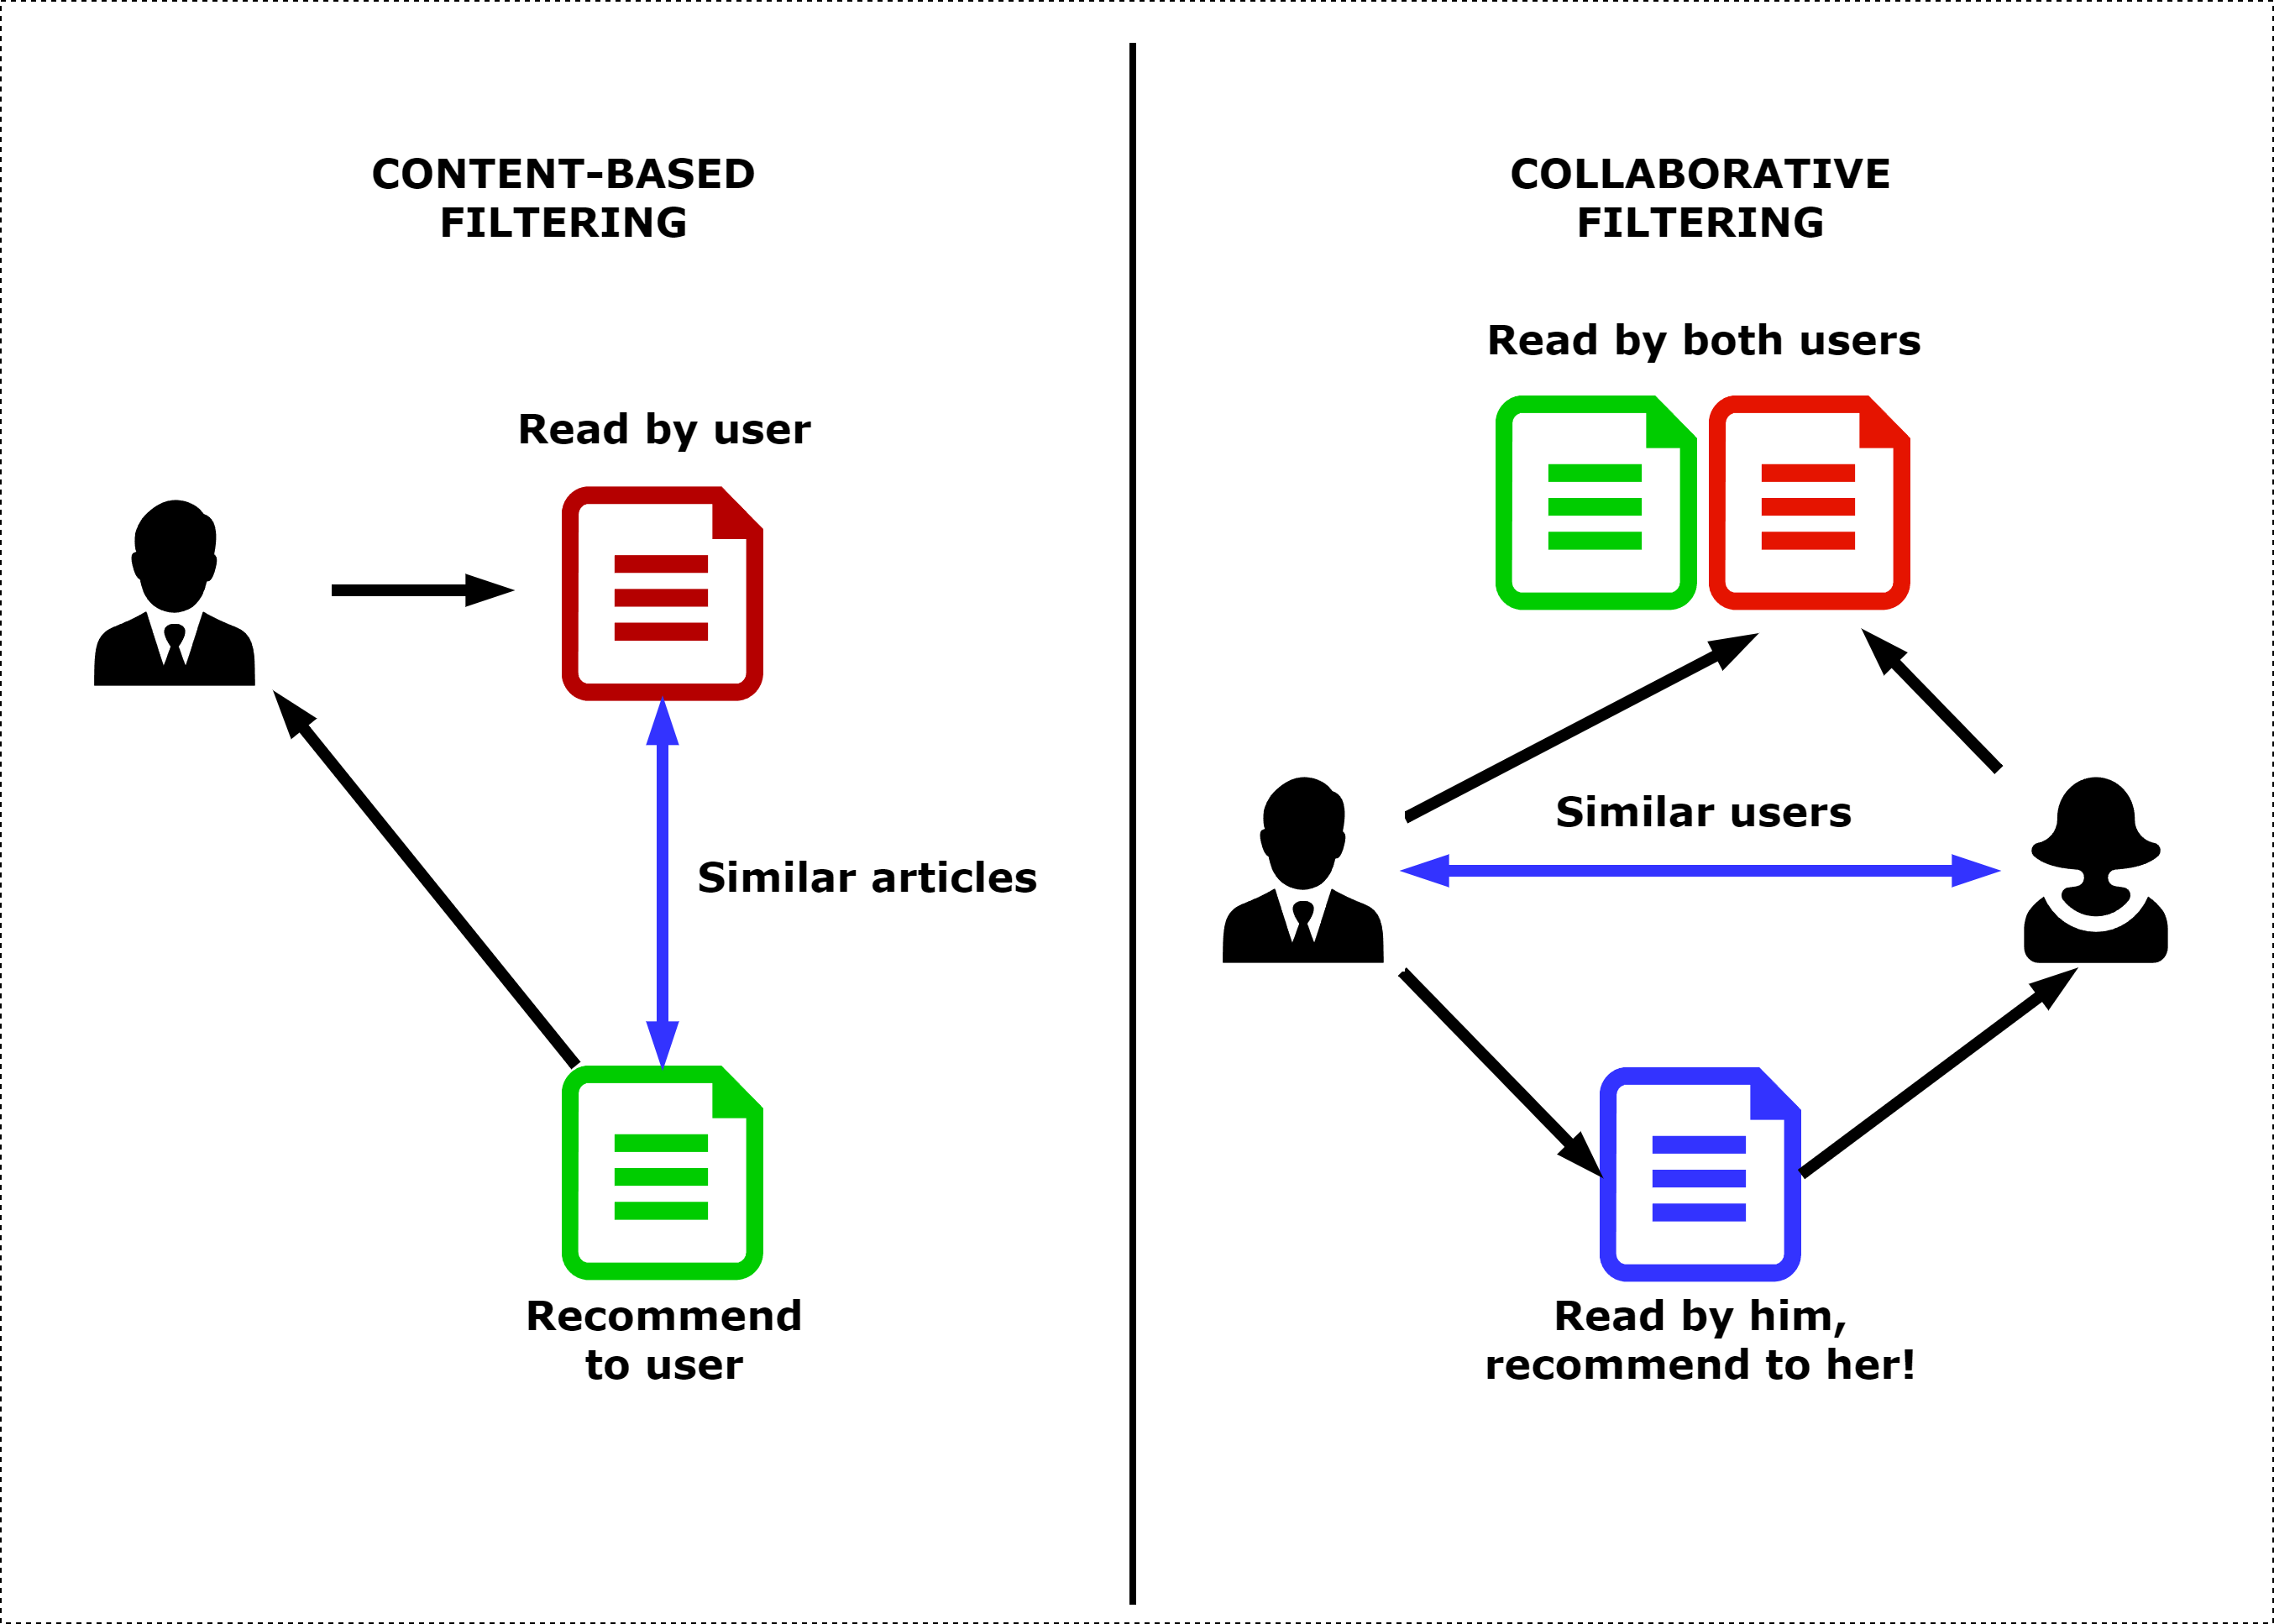
\includegraphics[width = 0.8\textwidth]{imgs/CF_CBF.png}
% %     \caption{Minh hoạ Lọc dựa trên nội dung và Lọc cộng tác}
% %     \label{fig:CF_CBF}
% % \end{figure}
% % \subsubsection{Lọc cộng tác}
% % Lọc cộng tác (Collaborative Filtering - CF) là một kỹ thuật phổ biến trong các hệ thống khuyến nghị, hoạt động dựa trên nguyên tắc "những người cùng sở thích sẽ có xu hướng thích những thứ tương tự nhau" (minh họa trong hình \ref{fig:CF_CBF}) \cite{cf2,cf3}. CF có thể được chia thành hai loại chính: dựa trên bộ nhớ (Memory-based) và dựa trên mô hình (Model-based).

% % \begin{enumerate}
% %     \item Lọc cộng tác dựa trên bộ nhớ (Memory-based): Phương pháp này tập trung vào việc tìm kiếm sự tương đồng giữa người dùng hoặc giữa các mục để đưa ra khuyến nghị. Ví dụ, trong kỹ thuật Lọc cộng tác người dùng-người dùng, hệ thống sẽ gợi ý các mục dựa trên những gì mà những người dùng có sở thích tương tự đã yêu thích hoặc đánh giá cao \cite{ncf1, ncf3}.
% %     \item Lọc cộng tác dựa trên mô hình (Model-based): Khác với phương pháp dựa trên bộ nhớ, cách tiếp cận này xây dựng một mô hình từ dữ liệu người dùng để dự đoán sở thích của họ. Một ví dụ điển hình là Phân tích ma trận (Matrix Factorization), một kỹ thuật phân tích dữ liệu đánh giá thành các yếu tố tiềm ẩn, đại diện cho sở thích của người dùng và đặc điểm của mục \cite{ncf2, ncf4}.
% % \end{enumerate}
% % \subsubsection{Lọc dựa trên nội dung}
% % Lọc Dựa trên nội dung (Content-based Filtering - CB) là một kỹ thuật khuyến nghị tập trung vào việc phân tích các đặc điểm nội tại của từng mục và sở thích của người dùng để đưa ra các đề xuất phù hợp. Điểm mấu chốt của phương pháp này nằm ở giả định rằng nếu người dùng yêu thích một mục cụ thể, họ cũng có xu hướng quan tâm đến những mục khác có nội dung tương đồng (như trong hình \ref{fig:CF_CBF}) \cite{cbf1,cbf2}. Ví dụ, nếu một người thường xuyên đọc các bài báo về học sâu, hệ thống có thể gợi ý cho họ những bài viết khác liên quan đến lĩnh vực này \cite{cbf, cbf1, cbf2}.


% % \subsubsection{Khuyến nghị tuần tự}
% % Gần đây, với sự tiến bộ trong các phương pháp học máy và học sâu, các hệ thống khuyến nghị tuần tự (Sequential Recommender Systems) đã nổi lên như một xu hướng mới, mang lại nhiều lợi ích và khả năng cải thiện trải nghiệm người dùng một cách đáng kể. Các mô hình khuyến nghị trong tuần tự tập trung vào thứ tự và ngữ cảnh của sản phẩm mà người dùng đã tương tác. Khoá luận này sẽ tập trung sử dụng mô hình khuyến nghị tuần tự đề xây dựng phương pháp đề xuất. Với hai mô hình cơ sở nổi bật được tập trung nghiên cứu là Self-Attentive Sequential Recommendation (SASRec) và Bidirectional Encoder Representations from Transformers for Recommendation (BERT4Rec).
% % \begin{figure}
% %     \centering
% %     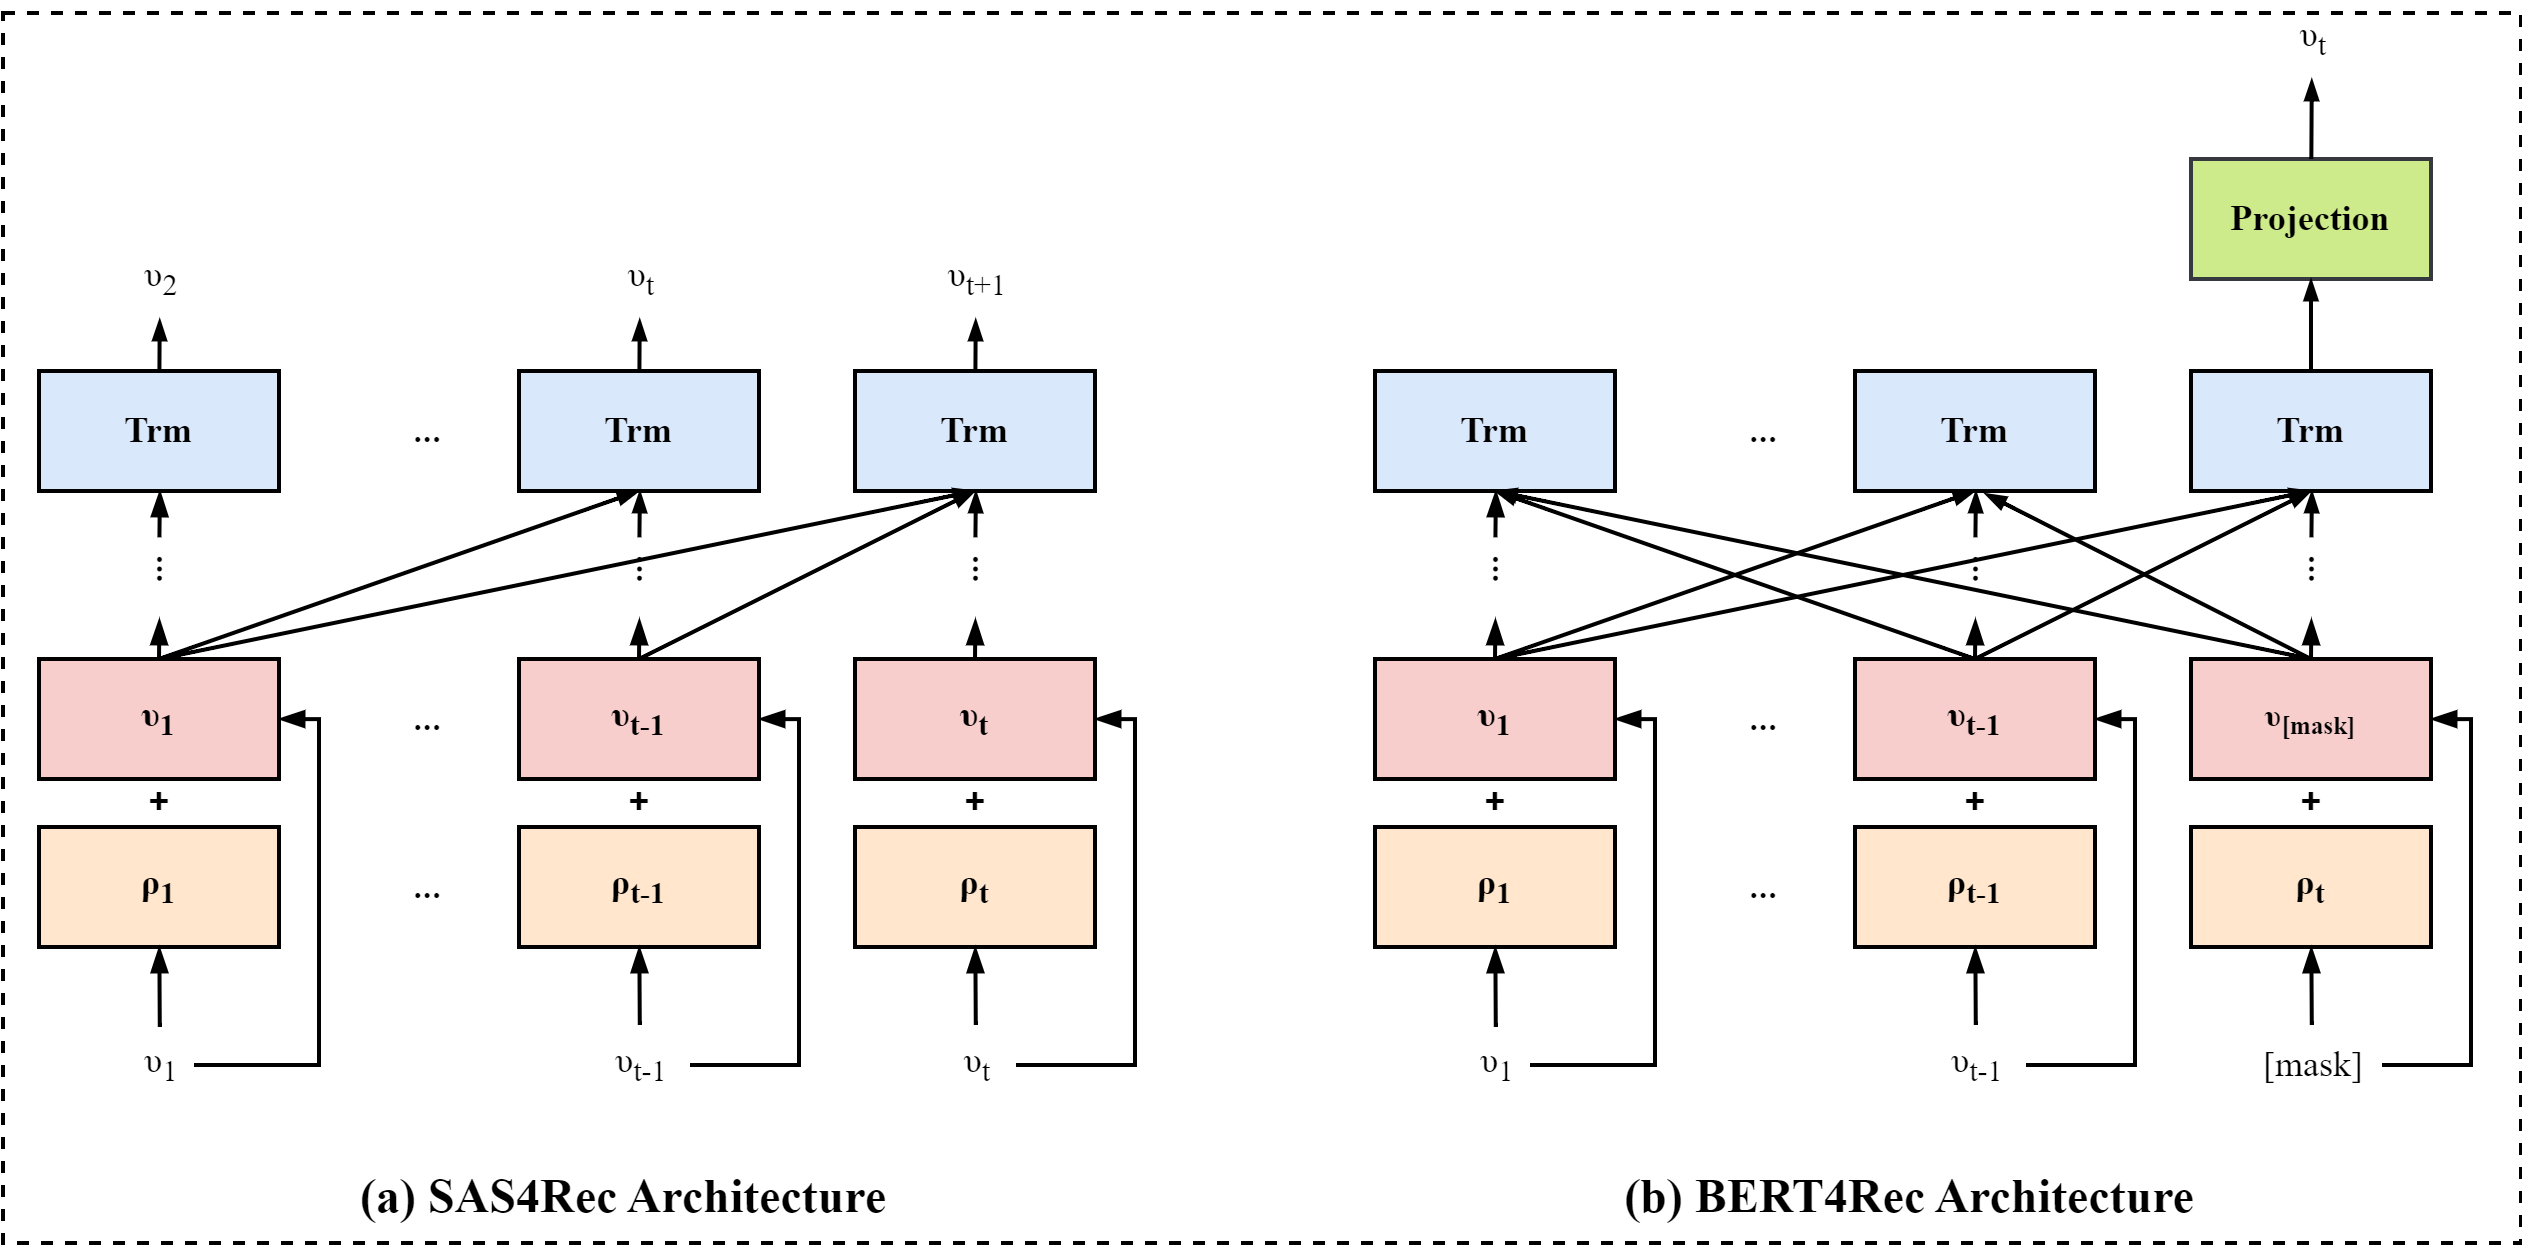
\includegraphics[width = \textwidth]{imgs/bert_sas_1.png}
% %     \caption{Kiến trúc của SASRec và BERT4Rec}
% %     \label{fig:bert_sas}
% % \end{figure}

% % \subsubsection{SASRec}
% % Được giới thiệu trong nghiên cứu \cite{sasrec}, SASRec là một trong những mô hình đầu tiên ứng dụng thành công Transformer vào bài toán khuyến nghị tuần tự. Như mô tả ở hình \ref{fig:bert_sas}a, điểm đặc biệt của SASRec nằm ở việc sử dụng cơ chế self-attention để nắm bắt các mối quan hệ phức tạp giữa các mục trong lịch sử tương tác của người dùng. Nhờ đó, mô hình có thể học được các biểu diễn phong phú và có ý nghĩa của từng mục, giúp dự đoán chính xác về mục tiếp theo mà người dùng có thể quan tâm. SASRec đã chứng minh được hiệu quả vượt trội so với các mô hình truyền thống như RNN và LSTM trong nhiều bài toán khuyến nghị tuần tự.
% % \subsubsection{BERT4Rec}
% % Được lấy cảm hứng từ mô hình BERT (Bidirectional Encoder Representations from Transformers), BERT4Rec được công bố trong nghiên cứu \cite{bert} với nhiệm vụ tận dụng khả năng của Transformer trong lĩnh vực hệ thống khuyến nghị. Khác với SASRec, ý tưởng chính của BERT4Rec là khai thác thông tin từ cả hai hướng (trước và sau) của chuỗi tương tác để xây dựng biểu diễn ngữ cảnh (như hình \ref{fig:bert_sas}b, cho phép mô hình nắm bắt được cả thông tin ngữ cảnh trước và sau của mỗi mục, từ đó hiểu rõ hơn về mối quan hệ giữa các mục và đưa ra các dự đoán chính xác hơn. BERT4Rec đã đạt được những kết quả ấn tượng trên nhiều tập dữ liệu, khẳng định vị thế của mình như một trong những mô hình hàng đầu trong lĩnh vực này.
% \subsubsection{Tổng kết}
% Tóm lại, các hệ thống khuyến nghị tuần tự đóng vai trò quan trọng trong việc mang đến trải nghiệm cá nhân hóa cho người dùng. Tuy nhiên, các mô hình này thường chỉ tập trung vào thông tin từ chuỗi hành vi của người dùng mà chưa tập trung vào việc khai thác thông tin đa chiều về các khóa học. Để giải quyết hạn chế này, nghiên cứu này đề xuất tích hợp HINs với BERT4Rec. Bằng cách khai thác các biểu diễn thực thể đa dạng thông qua HINs, mô hình kết hợp được cả đặc điểm nội dung và đặc điểm cấu trúc của các thực thể trong dữ liệu MOOCs. Sự tích hợp này hứa hẹn sẽ nâng cao đáng kể khả năng gợi ý các khái niệm kiến thức, nhờ vào việc tận dụng thông tin toàn diện từ nhiều nguồn khác nhau.

% \subsection{Các ứng dụng của lấy mẫu tiêu cực}
% Lấy mẫu tiêu cực (negative sampling) là một kỹ thuật lấy mẫu dữ liệu quan trọng, đặc biệt hiệu quả trong việc xử lý các tập dữ liệu mất cân bằng thường gặp trong các mô hình học máy như mạng nơ-ron và nhúng từ \cite{neg_1,neg_2}. Kỹ thuật này hoạt động bằng cách chọn lọc một tập hợp con các mẫu tiêu cực từ một phân phối xác định trước, thường sử dụng chiến lược lấy mẫu ngẫu nhiên. Tuy nhiên, việc lấy mẫu ngẫu nhiên không phải lúc nào cũng là lựa chọn tối ưu cho mọi nhiệm vụ. Trong lĩnh vực nhúng từ (như Word2Vec), negative sampling đã chứng minh được hiệu quả vượt trội trong việc giảm thiểu đáng kể khối lượng tính toán. Thay vì cập nhật trọng số dựa trên toàn bộ từ vựng, kỹ thuật này tập trung vào một tập hợp nhỏ các từ tiêu cực được lựa chọn cẩn thận, giúp tăng tốc độ huấn luyện và khả năng ứng dụng của mô hình nhúng từ, ngay cả với những bộ từ vựng lớn.

% Negative sampling có ứng dụng rộng rãi trong nhiều lĩnh vực, từ học máy, thị giác máy tính, xử lý ngôn ngữ tự nhiên đến khai thác dữ liệu và hệ thống gợi ý \cite{neg_1}. Có nhiều phương pháp negative sampling khác nhau, bao gồm static negative, hard negative và các phương pháp dựa trên GAN, mỗi phương pháp đều có ưu nhược điểm riêng. 
% Khoá luận này đề xuất một chiến lược lấy mẫu ngẫu nhiên mới với thông tin được tổng hợp bởi HINs. Nghiên cứu sẽ thực nghiệm để hiểu rõ tầm ảnh hưởng của việc áp dụng các chiến lược lấy mẫu ngẫu nhiên khác nhau khi xây dựng hệ thống khuyến nghị khoá học. Kết quả đánh giá sẽ cho thấy được rằng việc áp dụng chiến lược lấy mẫu ngẫu nhiên mà khoá luận đề xuất là tốt hơn so với các chiến lược được sử dụng trong các nghiên cứu trước đây như \cite{bert, sasrec, gru_ori}.

% \subsection{Mạng thông tin không đồng nhất}
% Mạng thông tin không đồng nhất (HINs) đã thu hút sự quan tâm lớn từ cộng đồng nghiên cứu do khả năng biểu diễn dữ liệu phong phú và đa dạng từ nhiều nguồn thông tin khác nhau. Các HINs không chỉ lưu trữ các loại đối tượng và liên kết khác nhau mà còn hỗ trợ các ứng dụng phân tích dữ liệu phức tạp, từ việc khai thác tri thức đến dự đoán và khuyến nghị. HINs là các mạng trong đó tồn tại nhiều loại đối tượng và liên kết, khác biệt với các mạng đồng nhất truyền thống nơi chỉ có một loại đối tượng và một loại liên kết duy nhất \cite{rlt_hin}. Cho phép HINs mô hình hóa mối quan hệ phức tạp giữa các thực thể khác nhau và hỗ trợ các ứng dụng trong nhiều lĩnh vực như mạng xã hội, khoa học dữ liệu, và y học. Khác với các mạng đồng nhất, nơi mà tất cả các đối tượng và liên kết đều cùng loại, HINs cung cấp một cấu trúc phong phú hơn, cho phép biểu diễn mối quan hệ phức tạp giữa các loại thực thể khác nhau \cite{rlt_hin2}. Các mạng đồng nhất thường không thể hiện được đầy đủ sự đa dạng và ngữ cảnh của dữ liệu, dẫn đến việc mất mát thông tin quan trọng khi mô hình hóa các hệ thống phức tạp.

% \subsubsection{Ưu điểm}
% \begin{itemize}
%     \item Biểu diễn thông tin phong phú: HINs có khả năng biểu diễn thông tin một cách chi tiết và đa dạng từ nhiều loại đối tượng và mối liên kết khác nhau, giúp cung cấp ngữ cảnh đầy đủ và chính xác hơn \cite{rlt_hin}.
    
%     \item Nâng cao khả năng phân tích: Khả năng khai thác các mối quan hệ đa dạng và gián tiếp giữa các đối tượng giúp HINs tăng cường khả năng phân tích và khai thác tri thức từ dữ liệu \cite{rlt_hin2}.
    
%     \item Cải thiện độ chính xác của khuyến nghị: Bằng cách tận dụng thông tin từ nhiều nguồn và mối quan hệ khác nhau, HINs giúp cải thiện đáng kể hiệu suất của các hệ thống khuyến nghị \cite{rlt_hin3}.
% \end{itemize}
% \subsubsection{Thách thức}
% \begin{itemize}
%     \item Độ phức tạp: Việc xây dựng và quản lý HINs đòi hỏi nhiều công sức và kỹ thuật hơn so với các mạng đồng nhất, do tính chất đa dạng và phức tạp của dữ liệu \cite{rlt_hin3}. Các phương pháp đặc biệt cần được phát triển để xử lý và khai thác hiệu quả dữ liệu từ HINs.
    
%     \item Khả năng mở rộng: Khả năng mở rộng của các mô hình HINs là một thách thức đáng kể do sự đa dạng và phức tạp của dữ liệu \cite{rlt_hin5}. Việc áp dụng HINs cho các tập dữ liệu lớn đòi hỏi các giải pháp tối ưu hóa và xử lý phân tán để đảm bảo hiệu suất và khả năng đáp ứng của mô hình.
% \end{itemize}

% HINs đại diện cho một bước tiến quan trọng trong việc khai thác và phân tích dữ liệu phức tạp. Nhờ khả năng biểu diễn và khai thác thông tin từ nhiều loại đối tượng và mối quan hệ, HINs đã mở ra nhiều cơ hội mới cho các ứng dụng phân tích dữ liệu và hệ thống khuyến nghị, đồng thời đặt ra những thách thức mới về mặt kỹ thuật và mô hình hóa.





% % Hệ thống gợi ý tuần tự trong MOOCs có khả năng xử lý hành vi theo thời gian của người dùng, tuy nhiên khả năng nắm bắt ngữ cảnh đa dạng còn hạn chế. Ngữ cảnh này bao gồm các khóa học, cấu trúc kiến thức, mối quan hệ tiền quyết, hồ sơ học viên và các thực thể liên quan khác. Để giải quyết vấn đề này, nghiên cứu gần đây đã tập trung vào việc áp dụng Mạng thông tin không đồng nhất (HIN) cho hệ thống gợi ý MOOCs.

% % HIN là loại mạng chứa nhiều loại nút và cạnh khác nhau, biểu diễn các mối quan hệ phức tạp trong dữ liệu. Chúng nắm bắt ý nghĩa sâu sắc của các đối tượng được cấu trúc và các kết nối trong mạng, cho phép phân tích và khai thác dữ liệu phức tạp hơn, cung cấp cái nhìn toàn diện về các cấu trúc và mối quan hệ ẩn giữ các thực thể\cite{hin_1}. Mặc dù HIN mang lại nhiều tiềm năng, việc áp dụng nó vào hệ thống gợi ý thực tiễn đặt ra nhiều thách thức. Một trong những thách thức chính là sự thưa thớt dữ liệu, nơi số lượng cạnh giữa các thực thể có thể không đủ để học các biểu diễn mạnh mẽ. Ngoài ra, việc thiết kế các phương pháp hiệu quả để tích hợp các nguồn dữ liệu đa dạng và các mối quan hệ phức tạp trong HINs có thể đòi hỏi tài nguyên tính toán đáng kể \cite{hin_2, hin_3, hin_4}.

% % Mô hình Heterogeneous Embedding for Recommendation (\textbf{HERec}) \cite{hin_5} đã cho thấy tiềm năng trong việc giải quyết những hạn chế này. HERec sử dụng các kỹ thuật nhúng để học các biểu diễn vector học viên, khóa học và các thực thể khác trong HINs. Biểu diễn mối quan hệ tự nhiên giữa các thực thể dựa trên kết nối của chúng trong mạng, cho phép HERec mô hình hóa hiệu quả các tương tác phức tạp giữa học viên, khóa học, khái niệm kiến thức và các khía cạnh quan trọng khác trong hệ sinh thái MOOCs. Cụ thể, HERec tận dụng các kỹ thuật dựa trên meta-path để khám phá các đường dẫn khác nhau trong HIN kết nối học viên với khóa học. Bằng cách xem xét những đường dẫn đa dạng này, HERec có thể nắm bắt được ngữ cảnh xung quanh các tương tác giữa học viên và khóa học, giúp cho các gợi ý được cá nhân hóa và phù hợp hơn cho người học.

% % Sự xuất hiện của mạng không đồng nhất và mô hình \textbf{HERec} đại diện cho một bước tiến đáng kể trong các hệ thống gợi ý MOOCs. Bằng cách nắm bắt mạng lưới phức tạp của các mối quan hệ trong hệ sinh thái MOOCs, HINs cung cấp một ngữ cảnh phong phú hơn để hiểu hành vi của người dùng. Kết hợp với hiệu quả của HERec trong việc học các biểu diễn có ý nghĩa từ mạng này, nó mở ra con đường phát triển các hệ thống gợi ý cá nhân hóa và tinh vi hơn cho các nền tảng MOOCs.

\section{Deep learning}

Sự trỗi dậy của học sâu (deep learning) trong những năm gần đây đã mở ra những hướng tiếp cận mới để khai thác tri thức từ các bộ dữ liệu lớn. Trong lĩnh vực giáo dục, Mạng nơ-ron nhân tạo (ANN) là một trong những kiến trúc nền tảng được ứng dụng rộng rãi nhất để phân tích hành vi người học. Với cấu trúc nhiều lớp mô phỏng não bộ, ANN thể hiện khả năng xử lý hiệu quả dữ liệu quy mô lớn. Các ứng dụng của nó rất đa dạng, từ việc dự báo kết quả học tập, xác định các hành vi bất thường có thể dẫn đến việc bỏ học, cho đến gợi ý các lộ trình học tập được cá nhân hóa \cite{waheed2020predicting, coelho2017deep}.

Bên cạnh ANN, các kiến trúc sâu hơn như Mạng Nơ-ron Sâu (DNNs) và đặc biệt là các mô hình lai ghép như CNN-LSTM đã chứng tỏ được hiệu quả vượt trội trong giai đoạn 2019-2023. Các kỹ thuật như Mạng tích chập (CNN) và Mạng bộ nhớ dài-ngắn (LSTM) khi được kết hợp có khả năng xử lý hiệu quả các dữ liệu giáo dục vốn có tính đa chiều và phi tuyến tính. Nhiều nghiên cứu trong giai đoạn này đã báo cáo độ chính xác trên 90\%, qua đó củng cố mạnh mẽ niềm tin về tiềm năng của học sâu trong việc dự đoán hành vi và kết quả học tập \cite{albreiki2021systematic}.

Sức mạnh kiến trúc lai CNN-LSTM nằm ở sự tổng hợp của hai năng lực bổ trợ cho nhau: Năng lực xử lý thông tin không gian của CNN và thông tin thời gian của LSTM. Nhờ đó, mô hình này có thể phân tích hiệu quả các dữ liệu học tập chứa cả yếu tố không gian (ví dụ: các loại tương tác khác nhau) và yếu tố thời gian (trình tự và thời điểm của các hành động đó). Điều này hữu ích cho các nhiệm vụ như dự báo điểm số, nhận diện nguy cơ bỏ học và hỗ trợ các quyết định sư phạm \cite{aljaloud2022deep}.

Để xử lý hiệu quả hơn nữa dữ liệu dạng chuỗi thời gian vốn rất phổ biến trong giáo dục trực tuyến, kiến trúc LSTM xếp chồng nhiều lớp (stacked LSTM), chẳng hạn như mô hình 4 lớp, đã được đề xuất. Việc xếp chồng các lớp LSTM cho phép mô hình học được các biểu diễn trừu tượng ở mức độ cao hơn, từ đó nắm bắt được các mẫu hành vi phức tạp và dài hạn qua nhiều phiên học. Do vậy, kiến trúc này tỏ ra rất hiệu quả trong việc phân tích quá trình học tập và dự báo các kết quả trong tương lai \cite{kukkar2023prediction, ren2023prediction}.

Một bước tiến xa hơn trong việc phân tích dữ liệu tuần tự là việc áp dụng LSTM hai chiều (BiLSTM), một kiến trúc có khả năng khai thác thông tin từ cả quá khứ và tương lai của chuỗi. Khi được tích hợp với cơ chế chú ý (attention mechanism), BiLSTM càng cho thấy ưu thế vượt trội. Cơ chế chú ý giúp mô hình tập trung vào những thời điểm hoặc hành vi quan trọng nhất trong chuỗi, những yếu tố có ảnh hưởng quyết định đến kết quả cuối cùng. Sự kết hợp này đã mang lại độ chính xác cao hơn đáng kể trong việc phân tích hành vi, mở đường cho việc thiết kế các hệ thống cảnh báo sớm và hỗ trợ học tập thông minh \cite{yousafzai2021student}.

Tóm lại, bức tranh ứng dụng học sâu trong lĩnh vực khai phá dữ liệu giáo dục rất đa dạng và không ngừng phát triển. Các kiến trúc từ ANN, DNN, CNN-LSTM, stacked LSTM, cho đến BiLSTM với cơ chế chú ý, đã tạo thành một bộ công cụ mạnh mẽ. Chúng không những là các công cụ dự đoán hiệu quả mà còn là phương tiện để khám phá bản chất phức tạp, đa chiều của hành vi học tập trong kỷ nguyên số.

% Một trong những mô hình học sâu đã nổi lên và khá nổi tiếng trong nghiên cứu hành vi người học là mạng nơ-ron nhân tạo (Artificial Neural Networks – ANN). Cơ chế ANNs khá giống cơ chế hoạt động của não bộ con người nhờ các lớp nơ-ron nhân tạo, thường bao gồm ba lớp cơ bản: lớp đầu vào, lớp ẩn và lớp đầu ra. ANNs có khả năng xử lý dữ liệu lớn và có hiệu quả trong việc dự đoán kết quả học tập, phát hiện hành vi bất thường của các học viên có nguy cơ không hoàn thành khóa học và gợi ý những lộ trình học tập tối ưu hóa cho từng cá nhân \cite{waheed2020predicting, coelho2017deep}.

% Bên cạnh ANNs, Deep Neural Networks – DNNs và các kiến trúc kết hợp như CNN-LSTM cũng được áp dụng rộng rãi trong bài toán giáo dục, đặc biệt trong giai đoạn 2019-2023. Sức mạnh của các kỹ thuật như mạng tích chập (Convolutional Neural Networks – CNNs), mạng ghi nhớ dài hạn (Long Short-Term Memory – LSTM) và các mô hình kết hợp để xử lý dữ liệu giáo dục có tính chất đa chiều và phi tuyến đã được nghiên cứu rất nhiều trong khoảng thời gian này. Những mô hình này thường đạt được độ chính xác rất cao, trong nhiều trường hợp vượt mốc 90\%, góp phần củng cố niềm tin vào khả năng áp dụng học sâu trong dự đoán học lực và hành vi học tập \cite{albreiki2021systematic}.

% Mô hình CNN-LSTM là sự kết hợp giữa khả năng trích xuất đặc trưng không gian của CNN và khả năng ghi nhớ tuần tự của LSTM. CNN-LSTM xử lý dữ liệu học tập có cả yếu tố không gian (chẳng hạn như các loại hành vi học tập khác nhau) và yếu tố thời gian (thứ tự và thời điểm thực hiện hành vi) rất hiệu quả. Chính vì đó, nó phục vụ cho các nhiệm vụ như dự đoán điểm số, xác định nguy cơ bỏ học và hỗ trợ ra quyết định giảng dạy \cite{aljaloud2022deep}.

% Đặc biệt, kiến trúc LSTM xếp chồng nhiều lớp (stacked LSTM), tiêu biểu là mô hình 4-layer-stacked, được thiết kế để khai thác dạng dữ liệu chuỗi thời gian thường phổ biến trong các hệ thống học tập trực tuyến. Việc xếp chồng nhiều lớp LSTM giúp mô hình có thể học được các đặc trưng trừu tượng hơn, đại diện cho mối liên hệ phức tạp giữa các hành vi học tập kéo dài qua nhiều phiên học.\cite{kukkar2023prediction, ren2023prediction}.

% Không dừng lại ở đó, các mô hình học sâu tiên tiến hơn như LSTM hai chiều (Bidirectional LSTM – BiLSTM) được quan tâm nhiều hơn nhờ khả năng khai thác thông tin từ cả quá khứ lẫn tương lai trong chuỗi thời gian. Khi kết hợp với cơ chế chú ý (attention mechanism), BiLSTM cho thấy ưu thế trong việc trích xuất biểu diễn từ dữ liệu chuỗi. Việc tích hợp BiLSTM với attention đã mang lại kết quả vô cùng khả quan, từ đó mở ra tiềm năng tích hợp vào các hệ thống dự đoán thông minh\cite{yousafzai2021student}.

% Tóm lại, Các kiến trúc như ANN, DNN, CNN-LSTM, stacked LSTM, và BiLSTM kết hợp với attention không chỉ đóng vai trò là công cụ dự đoán hiệu quả, mà còn góp phần quan trọng trong việc khám phá bản chất phức tạp và đa chiều của hành vi học tập trong môi trường số. Việc vận dụng những mô hình này một cách linh hoạt và sáng tạo sẽ là chìa khóa để giải quyết bài toán tỷ lệ bỏ học và cải thiện tỷ lệ hoàn thành các khóa học trực tuyến.